\documentclass[border=4pt,12pt]{standalone}
% House style for redrawn exam diagrams (diagram-v4: 0.4pt lines, filled -latex arrows, fine dashes; stipple and hatching drawn as real dots/lines (no PDF/SVG patterns, so they render in every browser and at any scale); transparent background). Every figure \input's this.
\usepackage{amsmath,amssymb}
\usepackage{txfonts}
\usepackage{pdfrender,xcolor}
% \halo{text}: label on shading. The shading stops just around each letter's outline (a thin knock-out that follows the
% glyphs, like the papers' typesetting), never a box. Owner: "I don't want a box around the text".
\newcommand{\halo}[1]{\leavevmode\rlap{\pdfrender{TextRenderingMode=2,LineWidth=2.2pt,LineJoinStyle=1,StrokeColor=white,FillColor=white}#1}#1}
\usepackage{tikz,pgfplots}
\pgfplotsset{compat=1.18}
\usetikzlibrary{arrows.meta,calc,angles,quotes,patterns,patterns.meta,intersections,positioning,decorations.markings,shapes.geometric}
% Stipple and hatching are drawn as actual dots / lines clipped to the region (path picture), NOT as pattern fills:
% SVG <pattern> fills vanish or blur when browsers scale the image, so the owner could not see the shading.
% Each dot is a 0.72pt square (keeps SVGs small; reads as a dot at print size). Dots sit on one global staggered grid, so neighbouring regions line up.
\makeatletter
\newdimen\ex@x \newdimen\ex@y \newdimen\ex@xa \newdimen\ex@ya \newdimen\ex@xb \newdimen\ex@yb \newcount\ex@row
\def\exam@stipplecolor{black!75}\def\exam@dotr{0.42pt}\def\exam@dotgap{2.5}
\def\ex@rowdots{\ifdim\ex@x<\ex@xb \pgfpathrectangle{\pgfqpoint{\dimexpr\ex@x-0.36pt\relax}{\dimexpr\ex@y-0.36pt\relax}}{\pgfqpoint{0.72pt}{0.72pt}}\advance\ex@x by \exam@dotgap pt\relax\expandafter\ex@rowdots\fi}
\def\exam@stipple{%
  \pgftransformreset% dots are sized in real points even inside scaled pictures
  \pgfpointanchor{path picture bounding box}{south west}\ex@xa=\pgf@x \ex@ya=\pgf@y
  \pgfpointanchor{path picture bounding box}{north east}\ex@xb=\pgf@x \ex@yb=\pgf@y
  \pgfsetfillcolor{\exam@stipplecolor}\pgfmathsetmacro\ex@h{\exam@dotgap/2}%
  \pgfmathtruncatemacro\ex@r{floor(\ex@ya/\ex@h)-1}\ex@row=\ex@r\relax
  \ex@y=\ex@r\dimexpr\ex@h pt\relax
  \loop\ifdim\ex@y<\ex@yb
    \pgfmathtruncatemacro\ex@c{floor(\ex@xa/\exam@dotgap)-1}\ex@x=\ex@c\dimexpr\exam@dotgap pt\relax
    \ifodd\ex@row \advance\ex@x by \ex@h pt\fi
    \ex@rowdots
    \advance\ex@y by \ex@h pt \advance\ex@row by 1
    \ifnum\numexpr\ex@row-(\ex@row/4)*4\relax=0 \pgfusepath{fill}\fi% flush every 4 rows: bounded TeX memory, few clip copies in the SVG
  \repeat\pgfusepath{fill}}
\newdimen\ex@d
\def\exam@hatch#1{% #1 = 1 for /, -1 for \ ; lines 45 degrees, 3pt apart
  \pgftransformreset
  \pgfpointanchor{path picture bounding box}{south west}\ex@xa=\pgf@x \ex@ya=\pgf@y
  \pgfpointanchor{path picture bounding box}{north east}\ex@xb=\pgf@x \ex@yb=\pgf@y
  \ex@d=\dimexpr\ex@yb-\ex@ya\relax \ex@x=\dimexpr\ex@xa-\ex@d\relax
  \loop\ifdim\ex@x<\ex@xb
    \ifnum#1>0 \pgfpathmoveto{\pgfqpoint{\ex@x}{\ex@ya}}\pgfpathlineto{\pgfqpoint{\dimexpr\ex@x+\ex@d\relax}{\ex@yb}}%
    \else \pgfpathmoveto{\pgfqpoint{\ex@x}{\ex@yb}}\pgfpathlineto{\pgfqpoint{\dimexpr\ex@x+\ex@d\relax}{\ex@ya}}\fi
    \advance\ex@x by 4.24pt
  \repeat
  \pgfsetlinewidth{0.4pt}\pgfsetstrokecolor{black}\pgfusepath{stroke}}
\def\examstipple{\exam@stipple}\def\examhatch{\exam@hatch}\def\examsetstipplecolor#1{\def\exam@stipplecolor{#1}}\def\examsetdotgap#1{\def\exam@dotgap{#1}}
\makeatother
% (legacy pattern kept for old files)
% staggered stipple like the NESA papers' dotted shading
\pgfdeclarepatternformonly{exam stipple}{\pgfpointorigin}{\pgfqpoint{2.2pt}{2.2pt}}{\pgfqpoint{2.2pt}{2.2pt}}{%
  \pgfpathcircle{\pgfqpoint{0.55pt}{0.55pt}}{0.42pt}\pgfpathcircle{\pgfqpoint{1.65pt}{1.65pt}}{0.42pt}\pgfusepath{fill}}
\tikzset{
  every picture/.style={line width=0.6pt, >={Latex[length=2mm,width=1.3mm]}},
  curve/.style={line width=0.6pt},
  open arrow/.style={-{Latex[length=2mm,width=1.3mm]}},  % owner: filled -latex heads everywhere, no open chevrons
  aux/.style={dash pattern=on 2pt off 1.5pt, line width=0.6pt},
  shade/.code={\def\exA{#1}\def\exB{none}\ifx\exA\exB\else\pgfkeysalso{fill=black!18}\fi},
  shade/.default=on,
  shade dots/.style={fill=none, path picture={\examstipple}},
  stipple color/.code={\examsetstipplecolor{#1}},
  stipple gap/.code={\examsetdotgap{#1}},
  shade dense dots/.style={fill=none, stipple gap=1.6, path picture={\examstipple}},
  shade hatch/.style={fill=none, path picture={\examhatch{1}}},
  shade hatch reverse/.style={fill=none, path picture={\examhatch{-1}}},
  shade solid/.style={fill=black},
  pt/.style={circle, fill, inner sep=1.1pt},
  open pt/.style={circle, draw, fill=white, inner sep=1.1pt},
}
\pgfplotsset{
  exam axes/.style={axis lines=middle, axis line style={->}, xlabel={$x$}, ylabel={$y$},
    xlabel style={anchor=west}, ylabel style={anchor=south}, tick label style={font=\small},
    every axis plot/.append style={line width=0.6pt, black}, samples=200, clip=false,
    enlargelimits=false, axis on top},
}

\begin{document}
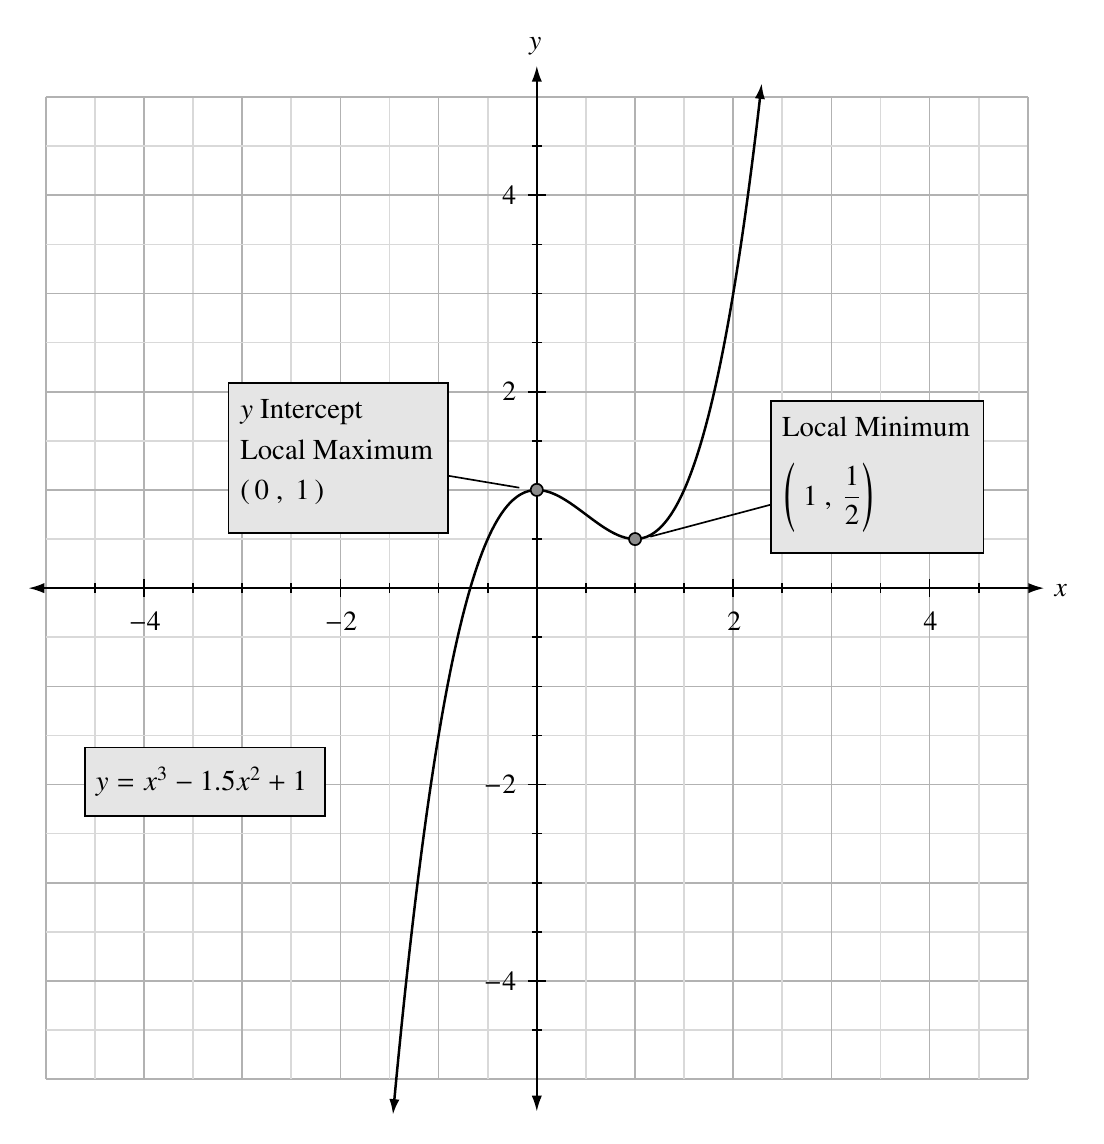
\begin{tikzpicture}[x=0.0127cm, y=-0.0127cm, font=\fontsize{10}{12}\selectfont, box/.style={draw, fill=black!10, inner sep=0pt}]
\draw[black!30] (132.2,76.2) -- (132.2,1058.8);
\draw[black!30] (132.2,1058.8) -- (1114.8,1058.8);
\draw[black!15] (181.4,76.2) -- (181.4,1058.8);
\draw[black!15] (132.2,1009.6) -- (1114.8,1009.6);
\draw[black!30] (230.5,76.2) -- (230.5,1058.8);
\draw[black!30] (132.2,960.5) -- (1114.8,960.5);
\draw[black!15] (279.6,76.2) -- (279.6,1058.8);
\draw[black!15] (132.2,911.4) -- (1114.8,911.4);
\draw[black!30] (328.8,76.2) -- (328.8,1058.8);
\draw[black!30] (132.2,862.2) -- (1114.8,862.2);
\draw[black!15] (377.9,76.2) -- (377.9,1058.8);
\draw[black!15] (132.2,813.1) -- (1114.8,813.1);
\draw[black!30] (427.0,76.2) -- (427.0,1058.8);
\draw[black!30] (132.2,764.0) -- (1114.8,764.0);
\draw[black!15] (476.1,76.2) -- (476.1,1058.8);
\draw[black!15] (132.2,714.9) -- (1114.8,714.9);
\draw[black!30] (525.2,76.2) -- (525.2,1058.8);
\draw[black!30] (132.2,665.8) -- (1114.8,665.8);
\draw[black!15] (574.4,76.2) -- (574.4,1058.8);
\draw[black!15] (132.2,616.6) -- (1114.8,616.6);
\draw[black!15] (672.6,76.2) -- (672.6,1058.8);
\draw[black!15] (132.2,518.4) -- (1114.8,518.4);
\draw[black!30] (721.8,76.2) -- (721.8,1058.8);
\draw[black!30] (132.2,469.2) -- (1114.8,469.2);
\draw[black!15] (770.9,76.2) -- (770.9,1058.8);
\draw[black!15] (132.2,420.1) -- (1114.8,420.1);
\draw[black!30] (820.0,76.2) -- (820.0,1058.8);
\draw[black!30] (132.2,371.0) -- (1114.8,371.0);
\draw[black!15] (869.1,76.2) -- (869.1,1058.8);
\draw[black!15] (132.2,321.9) -- (1114.8,321.9);
\draw[black!30] (918.2,76.2) -- (918.2,1058.8);
\draw[black!30] (132.2,272.8) -- (1114.8,272.8);
\draw[black!15] (967.4,76.2) -- (967.4,1058.8);
\draw[black!15] (132.2,223.6) -- (1114.8,223.6);
\draw[black!30] (1016.5,76.2) -- (1016.5,1058.8);
\draw[black!30] (132.2,174.5) -- (1114.8,174.5);
\draw[black!15] (1065.6,76.2) -- (1065.6,1058.8);
\draw[black!15] (132.2,125.4) -- (1114.8,125.4);
\draw[black!30] (1114.8,76.2) -- (1114.8,1058.8);
\draw[black!30] (132.2,76.2) -- (1114.8,76.2);
\draw[<->] (115,567.5) -- (1131,567.5);
\draw[<->] (623.5,1091) -- (623.5,45);
\draw (181.4,562.5) -- (181.4,572.5);
\draw (618.5,1009.6) -- (628.5,1009.6);
\draw (230.5,558.5) -- (230.5,576.5);
\draw (614.5,960.5) -- (632.5,960.5);
\draw (279.6,562.5) -- (279.6,572.5);
\draw (618.5,911.4) -- (628.5,911.4);
\draw (328.8,562.5) -- (328.8,572.5);
\draw (618.5,862.2) -- (628.5,862.2);
\draw (377.9,562.5) -- (377.9,572.5);
\draw (618.5,813.1) -- (628.5,813.1);
\draw (427.0,558.5) -- (427.0,576.5);
\draw (614.5,764.0) -- (632.5,764.0);
\draw (476.1,562.5) -- (476.1,572.5);
\draw (618.5,714.9) -- (628.5,714.9);
\draw (525.2,562.5) -- (525.2,572.5);
\draw (618.5,665.8) -- (628.5,665.8);
\draw (574.4,562.5) -- (574.4,572.5);
\draw (618.5,616.6) -- (628.5,616.6);
\draw (672.6,562.5) -- (672.6,572.5);
\draw (618.5,518.4) -- (628.5,518.4);
\draw (721.8,562.5) -- (721.8,572.5);
\draw (618.5,469.2) -- (628.5,469.2);
\draw (770.9,562.5) -- (770.9,572.5);
\draw (618.5,420.1) -- (628.5,420.1);
\draw (820.0,558.5) -- (820.0,576.5);
\draw (614.5,371.0) -- (632.5,371.0);
\draw (869.1,562.5) -- (869.1,572.5);
\draw (618.5,321.9) -- (628.5,321.9);
\draw (918.2,562.5) -- (918.2,572.5);
\draw (618.5,272.8) -- (628.5,272.8);
\draw (967.4,562.5) -- (967.4,572.5);
\draw (618.5,223.6) -- (628.5,223.6);
\draw (1016.5,558.5) -- (1016.5,576.5);
\draw (614.5,174.5) -- (632.5,174.5);
\draw (1065.6,562.5) -- (1065.6,572.5);
\draw (618.5,125.4) -- (628.5,125.4);
\node at (231.5,601) {$-4$};
\node[anchor=east] at (613,960.5) {$-4$};
\node at (428.0,601) {$-2$};
\node[anchor=east] at (613,764.0) {$-2$};
\node at (821.0,601) {$2$};
\node[anchor=east] at (613,371.0) {$2$};
\node at (1017.5,601) {$4$};
\node[anchor=east] at (613,174.5) {$4$};
\node at (622,25) {$y$};
\node at (1147,570) {$x$};
\draw[<->,line width=0.9pt, smooth, samples=90, domain=-1.465:2.29, variable=\t] plot ({623.5+98.25*\t},{567.5-98.25*(\t*\t*\t-1.5*\t*\t+1)});
\filldraw[fill=black!45] (623.5,469.2) circle (2.2pt);
\filldraw[fill=black!45] (721.8,518.4) circle (2.2pt);
\draw[box] (315,362) rectangle (534.5,512.5);
\draw (534.5,455) -- (606,467);
\node[anchor=north west, align=left, inner sep=0pt, font=\fontsize{10.4}{14.6}\selectfont] at (326,378) {$y$ Intercept\\Local Maximum\\$(\,0\ ,\ 1\,)$};
\draw[box] (857.5,380) rectangle (1070.5,532.5);
\draw (857.5,484) -- (737,516);
\node[anchor=north west, inner sep=0pt, font=\fontsize{10.4}{14}\selectfont] at (868,395) {Local Minimum};
\node[font=\fontsize{10.4}{14}\selectfont] at (916,477) {$\left(\ 1\ ,\,\dfrac{1}{2}\right)$};
\draw[box] (171.5,727) rectangle (411.5,795.5);
\node[font=\fontsize{10.4}{14}\selectfont] at (288,761) {$y=x^3-1.5x^2+1$};
\end{tikzpicture}
\end{document}
